\documentclass[a4paper,landscape]{article}
\usepackage[margin=1cm]{geometry}
\usepackage{tikz}

\newcommand\innerEps{0.2mm}
\newcommand\norm{1}
\newcommand\flip{-1}
\newcommand\vflap[4]
{
\draw (#1, #2)
  -- ++(#4 * 0.5, -0.5)
  -- ++(0, -#3 + 1)
  -- ++(#4 * -0.5, -0.5)
  -- cycle
  ;
}

\begin{document}
\pagestyle{empty}
\begin{tikzpicture}
  [ remember picture
  , overlay
  , line width=0.02cm
  ]

\draw (0,0)
  rectangle ++(5,-4)
  rectangle ++(5,4)
  rectangle ++(5,-4)
  rectangle ++(5,4)
  ;
\vflap{0}{0}{4}{\flip}
\draw[dotted] (0,-1) -- ++(20,0);
\draw[dotted] (      2.5,-1) -- ++(0,-3);
\draw[dotted] (5   + 2.5,-1) -- ++(0,-3);
\draw[dotted] (2*5 + 2.5,-1) -- ++(0,-3);
\draw[dotted] (3*5 + 2.5,-1) -- ++(0,-3);

\begin{scope}[yshift=-5cm]
\draw (0, 0)
  rectangle ++(5,-3)
  ;
\draw (2.5, 0) -- ++(0, -3/2);
\vflap{0}{0}{3}{\flip}
\vflap{5}{0}{3}{\norm}
\end{scope}

\begin{scope}[yshift=-5cm, xshift=7cm]
\draw (0, 0)
  rectangle ++(5,-3)
  ;
\draw (2.5, -3/2) -- ++(0, -3/2);
\vflap{0}{0}{3}{\flip}
\vflap{5}{0}{3}{\norm}
\end{scope}

\begin{scope}[yshift=-9cm]
\draw (1, 0)
  rectangle ++(5cm - \innerEps,-1)
  rectangle ++(-5cm + \innerEps,-5cm + \innerEps)
  rectangle ++(5cm - \innerEps,-1)
  ;
\draw (0, -1)
  rectangle ++(1,-5cm + \innerEps)
  ;
\draw (6cm - \innerEps, -1)
  rectangle ++(1,-5cm + \innerEps)
  ;
\end{scope}

\end{tikzpicture}
\end{document}
